% tikzpicture starts at line 2115 of input.tex
\documentclass{standalone}

\usepackage{amsthm, amsmath}

% Prevent the eventual "Too many alphabets" error
\newcommand\hmmax{0}
\newcommand\bmmax{0}

\RequirePackage{notomath}
\RequirePackage{inter}
\RequirePackage[scaled=0.85]{DejaVuSansMono}
\def\bfseries@rm{sb}

\DeclareMathVersion{sansmath}
\SetSymbolFont{operators}{sansmath}{OT1}{NotoSans-TLF}{m}{n}
\SetSymbolFont{letters}{sansmath}{OML}{notosansmi}{m}{it}
\SetMathAlphabet\mathbf{sansmath}{OT1}{NotoSans-TLF}{b}{n}
\SetMathAlphabet\mathsf{sansmath}{OT1}{NotoSans-TLF}{m}{n}
\SetMathAlphabet\mathit{sansmath}{OT1}{NotoSans-TLF}{m}{it}

\DeclareMathVersion{sansmathbold}
\SetSymbolFont{operators}{sansmathbold}{OT1}{NotoSans-TLF}{b}{n}
\SetSymbolFont{letters}{sansmathbold}{OML}{notosansmi}{b}{it}
\SetSymbolFont{symbols}{sansmathbold}{LMS}{ntxsy}{b}{n}
\SetMathAlphabet\mathbf{sansmathbold}{OT1}{NotoSans-TLF}{b}{n}
\SetMathAlphabet\mathsf{sansmathbold}{OT1}{NotoSans-TLF}{b}{n}
\SetMathAlphabet\mathit{sansmathbold}{OT1}{NotoSans-TLF}{b}{it}


% Upright Greek letters uppercase
\DeclareMathSymbol{\Gamma}{\mathord}{operators}{0}
\DeclareMathSymbol{\Delta}{\mathord}{operators}{1}
\DeclareMathSymbol{\Theta}{\mathord}{operators}{2}
\DeclareMathSymbol{\Lambda}{\mathord}{operators}{3}
\DeclareMathSymbol{\Xi}{\mathord}{operators}{4}
\DeclareMathSymbol{\Pi}{\mathord}{operators}{5}
\DeclareMathSymbol{\Sigma}{\mathord}{operators}{6}
\DeclareMathSymbol{\Upsilon}{\mathord}{operators}{7}
\DeclareMathSymbol{\Phi}{\mathord}{operators}{8}
\DeclareMathSymbol{\Psi}{\mathord}{operators}{9}
\DeclareMathSymbol{\Omega}{\mathord}{operators}{10}

% Italic Greek letters lowercase
\DeclareMathSymbol{\alpha}{\mathord}{letters}{11}
\DeclareMathSymbol{\beta}{\mathord}{letters}{12}
\DeclareMathSymbol{\gamma}{\mathord}{letters}{13}
\DeclareMathSymbol{\delta}{\mathord}{letters}{14}
\DeclareMathSymbol{\epsilon}{\mathord}{letters}{15}
\DeclareMathSymbol{\zeta}{\mathord}{letters}{16}
\DeclareMathSymbol{\eta}{\mathord}{letters}{17}
\DeclareMathSymbol{\theta}{\mathord}{letters}{18}
\DeclareMathSymbol{\iota}{\mathord}{letters}{19}
\DeclareMathSymbol{\kappa}{\mathord}{letters}{20}
\DeclareMathSymbol{\lambda}{\mathord}{letters}{21}
\DeclareMathSymbol{\mu}{\mathord}{letters}{22}
\DeclareMathSymbol{\nu}{\mathord}{letters}{23}
\DeclareMathSymbol{\xi}{\mathord}{letters}{24}
\DeclareMathSymbol{\pi}{\mathord}{letters}{25}
\DeclareMathSymbol{\rho}{\mathord}{letters}{26}
\DeclareMathSymbol{\sigma}{\mathord}{letters}{27}
\DeclareMathSymbol{\tau}{\mathord}{letters}{28}
\DeclareMathSymbol{\upsilon}{\mathord}{letters}{29}
\DeclareMathSymbol{\phi}{\mathord}{letters}{30}
\DeclareMathSymbol{\chi}{\mathord}{letters}{31}
\DeclareMathSymbol{\psi}{\mathord}{letters}{32}
\DeclareMathSymbol{\omega}{\mathord}{letters}{33}
\DeclareMathSymbol{\varepsilon}{\mathord}{letters}{34}
\DeclareMathSymbol{\vartheta}{\mathord}{letters}{35}
\DeclareMathSymbol{\varpi}{\mathord}{letters}{36}
\DeclareMathSymbol{\varrho}{\mathord}{letters}{37}
\DeclareMathSymbol{\varsigma}{\mathord}{letters}{38}
\DeclareMathSymbol{\varphi}{\mathord}{letters}{39}

% Change font tracking
\RequirePackage[letterspace=150]{microtype}

% Page breaking
\widowpenalty=10000
\clubpenalty=10000

%%%% Author's definition can start here

\usepackage{tikz}
\usepackage{tkz-graph}
\usepackage{mathdots}
\usepackage{dsfont}
\usetikzlibrary{shapes}

\DeclareMathOperator{\spn}{span}
\DeclareMathOperator{\tr}{tr}
\DeclareMathOperator{\rr}{\mathbb{R}}
\DeclareMathOperator{\cc}{\mathbb{C}}
\DeclareMathOperator{\arity}{arity}
\DeclareMathOperator{\vk}{\mathbf{K}}
\DeclareMathOperator{\vl}{\mathbf{L}}
\DeclareMathOperator{\vg}{\mathbf{G}}
\DeclareMathOperator{\vx}{\mathbf{x}}
\DeclareMathOperator{\vy}{\mathbf{y}}
\DeclareMathOperator{\vz}{\mathbf{z}}
\DeclareMathOperator{\va}{\mathbf{a}}
\DeclareMathOperator{\vb}{\mathbf{b}}
\DeclareMathOperator{\vq}{\mathbf{Q}}
\DeclareMathOperator{\vr}{\mathbf{R}}
\DeclareMathOperator{\vrr}{\mathbf{r}}
\DeclareMathOperator{\vc}{\mathbf{C}}
\DeclareMathOperator{\vcc}{\mathbf{c}}
\DeclareMathOperator{\vj}{\mathbf{J}}
\DeclareMathOperator{\vjj}{\mathbf{j}}
\DeclareMathOperator{\ic}{\mathcal{I}}
\DeclareMathOperator{\fc}{\mathcal{F}}
\DeclareMathOperator{\gc}{\mathcal{G}}
\DeclareMathOperator{\gk}{\mathfrak{G}_{\mathcal{F}}}
\DeclareMathOperator{\qk}{\mathfrak{Q}_{\mathcal{F}}}
\DeclareMathOperator{\stab}{Stab}
\newcommand{\tcwd}[1]{\left\langle #1 \right\rangle_{+, \circ, \otimes ,\top}}
\newcommand{\tcwdn}[1]{\left\langle #1 \right\rangle_{\circ, \otimes ,\top}}
\DeclareMathOperator{\holant}{Holant}
\DeclareMathOperator{\plholant}{Pl-Holant}
\DeclareMathOperator{\csp}{\#CSP}
\DeclareMathOperator{\qut}{Qut}
\DeclareMathOperator{\aut}{Aut}
\DeclareMathOperator{\eq}{\mathcal{EQ}}
\DeclareMathOperator{\geneq}{\mathcal{GEQ}}

\renewcommand*{\VertexSmallMinSize}{6pt}
% draw edges with diamonds in tikz
\newcommand{\DEdge}[2]{
    \draw[thick] (#1) -- (#2) node[draw, fill=white, kite, kite vertex angles = 120, minimum size = 4pt, inner sep = 1pt, pos=0.3, sloped] {};
}


\begin{document}
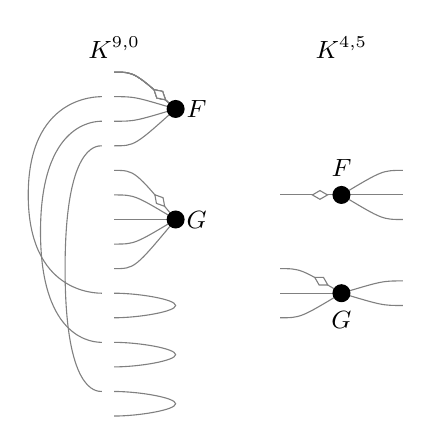
\begin{tikzpicture}[scale=.78]
    \tikzstyle{every node}=[font=\small]
    \GraphInit[vstyle=Classic]
    \SetUpEdge[style=-]
    \SetVertexMath

    % arm y coordinates
    \def\ysh{0.4}
    \def\vx{0}
    \def\xf{2.7}
    \def\wlen{1}
    \def\wgap{0.2}

    % G wires
    \draw[thin, color=gray] (\vx-\wlen, 3*\ysh) .. controls (\vx-\wlen+\wlen/3,3*\ysh) .. (\vx,1*\ysh) node[draw, fill=white, kite, kite vertex angles = 120, minimum size = 3pt, inner sep = 1pt, pos=0.85, sloped] {};
    \foreach \y in {-1,...,2} {
    \draw[thin, color=gray] (\vx-\wlen, \y*\ysh) .. controls (\vx-\wlen+\wlen/3,\y*\ysh) .. (\vx,1*\ysh);
    % F wires
    \draw[thin, color=gray] (\vx-\wlen, 7*\ysh) .. controls (\vx-\wlen+\wlen/3,7*\ysh) .. (\vx,5.5*\ysh) node[draw, fill=white, kite, kite vertex angles = 120, minimum size = 3pt, inner sep = 1pt, pos=0.85, sloped] {};
    }
    \foreach \y in {4,...,6} {
        \draw[thin, color=gray] (\vx-\wlen, \y*\ysh) .. controls (\vx-\wlen+\wlen/3,\y*\ysh) .. (\vx,5.5*\ysh);
    }
    % I wires
    \foreach \y in {-2,-4,-6} {
        \draw[thin, color=gray] (\vx-\wlen,\y*\ysh) .. controls
        +(0.4,0) and +(0,0.1) ..
        (\vx,{(\y-0.5)*\ysh}) .. controls
        +(0,-0.1) and +(0.4,0) ..
        (\vx-\wlen,{(\y-1)*\ysh});
    }

    \Vertex[x=\vx,y=1*\ysh,L={G},Ldist=-0.1cm]{g}
    \Vertex[x=\vx,y=5.5*\ysh,L={F},Ldist=-0.1cm]{f}

    % connecting wires
    \foreach \high/\low/\m in {4/-6/0.6,5/-4/1.0,6/-2/1.2} {
        \draw[thin, color=gray] (\vx-\wlen-\wgap,\high*\ysh) .. controls
        (\vx-\wlen-\wgap-0.1,\high*\ysh) and (\vx-\wlen-\wgap-\m,\high*\ysh) ..
        (\vx-\wlen-\wgap-\m,{(\high+\low)/2*\ysh}) .. controls
        (\vx-\wlen-\wgap-\m,\low*\ysh) and (\vx-\wlen-\wgap-0.1,\low*\ysh) ..
        (\vx-\wlen-\wgap,\low*\ysh);
    }
    \node at (\vx+1,0) {$\rightsquigarrow$};

    \node at (\xf,8*\ysh) {$K^{4,5}$};
    \node at (\vx-\wlen,8*\ysh) {$K^{9,0}$};

    % pivoted gadget
    \draw[thin, color=gray] (\xf-\wlen,2*\ysh) -- (\xf,2*\ysh) node[draw, fill=white, kite, kite vertex angles = 120, minimum size = 3pt, inner sep = 1pt, pos=0.65, sloped] {};
    \foreach \y in {1,2,3} {
        \draw[thin, color=gray] (\xf,2*\ysh) .. controls (\xf+2*\wlen/3,\y*\ysh) .. (\xf+\wlen,\y*\ysh);
    }

    \draw[thin, color=gray] (\xf,-2*\ysh) .. controls (\xf-2*\wlen/3,-1*\ysh) .. (\xf-\wlen,-1*\ysh) node[draw, fill=white, kite, kite vertex angles = 120, minimum size = 3pt, inner sep = 1pt, pos=0.2, sloped] {};
    \foreach \y in {-2,-3} {
        \draw[thin, color=gray] (\xf,-2*\ysh) .. controls (\xf-2*\wlen/3,\y*\ysh) .. (\xf-\wlen,\y*\ysh);
    }
    \foreach \y in {-1.5,-2.5} {
        \draw[thin, color=gray] (\xf,-2*\ysh) .. controls (\xf+2*\wlen/3,\y*\ysh) .. (\xf+\wlen,\y*\ysh);
    }
    % \draw[thin, color=gray] (\xg,4.5*\ysh) .. controls (\xg+2*\wlen/3,3.5*\ysh) .. (\xg+\wlen,3.5*\ysh);
    \Vertex[x=\xf,y=2*\ysh,L={F},Lpos=90]{ff}
    \Vertex[x=\xf,y=-2*\ysh,L={G},Lpos=270]{gg}
\end{tikzpicture}

    \pagestyle{empty}
    \centering

 

\end{document}
%%% Local Variables:
%%% mode: latex
%%% TeX-master: t
%%% End:
